\documentclass{article}
\usepackage{graphicx, amsmath, amssymb, mathtools, fancyhdr}

\graphicspath{{Images/}}

\setlength{\oddsidemargin}{0in}
\setlength{\textwidth}{6.5in}
\setlength{\topmargin}{-.55in}
\setlength{\textheight}{9in}
\pagestyle{fancy}

\fancyfoot{}
\fancyhead[R]{\thepage}
\fancyhead[L]{MAE 5131}


\begin{document}

\begin{center}
    {\huge CFD Homework 1}
    \vspace{0.5cm}

    {\Large Michael Nameika}
    \vspace{0.33cm}

    {\large 9/5/24}
\end{center}

\begin{itemize}
    \item[\textbf{1}.] Determine the mathematical character (hyperbolic, parabolic, or elliptic) of the system of the equations below.
    \begin{align*}
        \beta^2\frac{\partial u}{\partial x} - \frac{\partial v}{\partial y} &= 0\\
        \frac{\partial v}{\partial x} - \frac{\partial u}{\partial y} &= 0
    \end{align*}
    \textit{Soln.} Begin by dividing the first equation by $\beta^2$:
    \[\frac{\partial u}{\partial x} - \frac{1}{\beta^2}\frac{\partial v}{\partial y} = 0.\]
    Writing the system of PDEs as a linear system, we find
    \[\frac{\partial }{\partial x} \begin{pmatrix}
        u\\
        v
    \end{pmatrix} + \begin{pmatrix}
        0 & -\frac{1}{\beta^2}\\
        -1 & 0
    \end{pmatrix}\frac{\partial}{\partial y}\begin{pmatrix}
        u\\
        v
    \end{pmatrix} = \begin{pmatrix}
        0\\
        0
    \end{pmatrix}.\]
    Let 
    \[A = \begin{pmatrix}
        0 & -\frac{1}{\beta^2}\\
        -1 & 0
    \end{pmatrix}.\]
    We can classify our system of PDEs by inspecting the eigenvalues of $A$. Let $\lambda$ an eigenvalue of $A$. Then we want
    \[\text{det}(A - \lambda I) = 0\]
    where $I$ is the $2 \times 2$ identity matrix. That is,
    \begin{align*}
        \text{det}(A - \lambda I) &= \left|\begin{matrix}
            -\lambda & -\frac{1}{\beta^2}\\
            -1 & -\lambda
        \end{matrix}\right|\\
        &= \lambda^2 - \frac{1}{\beta^2} = 0\\
        \implies \lambda &= \pm \frac{1}{\beta}.
    \end{align*}
    Thus, $\lambda_1 = \frac{1}{\beta}, \lambda_2 = -\frac{1}{\beta} \in \mathbb{R}$ hence the system of PDEs is \textbf{hyperbolic}.
\pagebreak


\item[\textbf{2}.] 
    \begin{itemize}
        \item[a)] \underline{Verify} the solution of the following heat equation
        \[\frac{\partial u}{\partial t} = \frac{\partial^2u}{\partial x^2}\]
        with boundary conditions $u(t,0) = 0$, $u(t,1) = 0$ and initial distribution
        \[u(0,x) = \sin(2\pi x)\]
        is
        \[u(x,t) = 2\sum_{n = 1}^{\infty} \left(\int_0^1 \sin(2\pi x)\sin(n\pi x)dx\right)e^{-n^2 \pi^2t}\sin(n\pi x).\]
        Note this problem only asks to verify the solution provided.
        \newline\newline
    \textit{Soln.} Note that since $u(x,t)$ is a Fourier series, care must be taken when differentiating $u(x,t)$. That is to say, we must prove why we can term-by-term differentiate the series expansion for $u(x,t)$. Notice 
    \begin{align*}
        |u(x,t)| &= 2\left|\sum_{n = 1}^{\infty} \left(\int_0^1\sin(2\pi x)\sin(n \pi x)dx\right)e^{-n^2 \pi^2t}\sin(n \pi x)\right|\\
        &\leq 2\sum_{n=1}^{\infty} \left(\int_0^1|\sin(2\pi x)\sin(n \pi x)|dx\right)e^{-n^2 \pi^2 t}|\sin(n\pi x)|\\
        &\leq 2\sum_{n = 1}^{\infty} e^{-n^2 \pi^2t}.
    \end{align*}
    Note that for a fixed $t > 0$, we have that the series converges uniformly in $x$ by geometric series. To show that the series converges uniformly in $t$, notice that on the interval $t \in [\varepsilon, T]$ for some $\varepsilon > 0$, $T$ sufficiently large, 
    \[\sum_{n = 1}^{\infty} e^{-n^2\pi^2 t}\]
    converges uniformly on $[\varepsilon,T]$. Taking $\varepsilon \to 0$ gives uniform convergence for all $t > 0$. Thus, we may term-by-term differentiate in $t$. Now, differentiating:
    \begin{align*}
        \frac{\partial u}{\partial x} &= 2\frac{\partial}{\partial x}\sum_{n = 1}^{\infty} \left(\int_0^1\sin(2\pi y)\sin(n\pi y)dy\right)e^{-n^2\pi^2t}\sin(n\pi x)\\
        &= 2\sum_{n = 1}^{\infty} \left(\int_0^1 \sin(2\pi y) \sin(n \pi y)dy\right)e^{-n^2\pi^2t}(n\pi)\cos(n\pi x)\\
        \implies \frac{\partial^2u}{\partial x^2} &= 2\sum_{n = 1}^{\infty} \left(\int_0^1 \sin(2\pi y)\sin(n\pi y)dy \right)e^{-n^2\pi^2t}(-n^2\pi^2)\sin(n\pi x)
    \end{align*}
    and 
    \begin{align*}
        \frac{\partial u}{\partial t} &= 2\frac{\partial}{\partial t}\sum_{n = 1}^{\infty} \left(\int_0^1 \sin(2\pi y)\sin(n\pi y)dy\right) (-n^2\pi^2t)e^{-n^2\pi^2t} \sin(n\pi x)\\
        &= \frac{\partial^2u}{\partial x^2}.
    \end{align*}
    Further, notice 
    \begin{align*}
        u(0,t) &= 2\sum_{n = 1}^{\infty} \left(\int_0^1\sin(2\pi y)\sin(n\pi y)dy\right)e^{-n^2\pi^2t}\sin(0)\\
        &= 0
    \end{align*}
    and
    \begin{align*}
        u(1,t) &= 2\sum_{n = 1}^{\infty} \left(\int_0^1\sin(2\pi y)\sin(n \pi y)dy\right) e^{-n^2\pi^2 t}\sin(n\pi)\\
        &= 0.
    \end{align*}
    Now, using the fact that
    \[\int_0^1\sin(2\pi y)\sin(n\pi y)dy = \begin{cases}
        0 & n \neq 2\\
        \frac{1}{2} & n = 2
    \end{cases}\]
    so that 
    \[u(x,0) = \sin(2\pi x).\]
    Thus, the given Fourier series satisfies the PDE.
   

    \item[b)] Graph the above solution by numerically approximating the integral in the interval of $0 \leq x \leq 1$, $0 < t < 0.2$.
    \newline\newline
    \begin{center}
        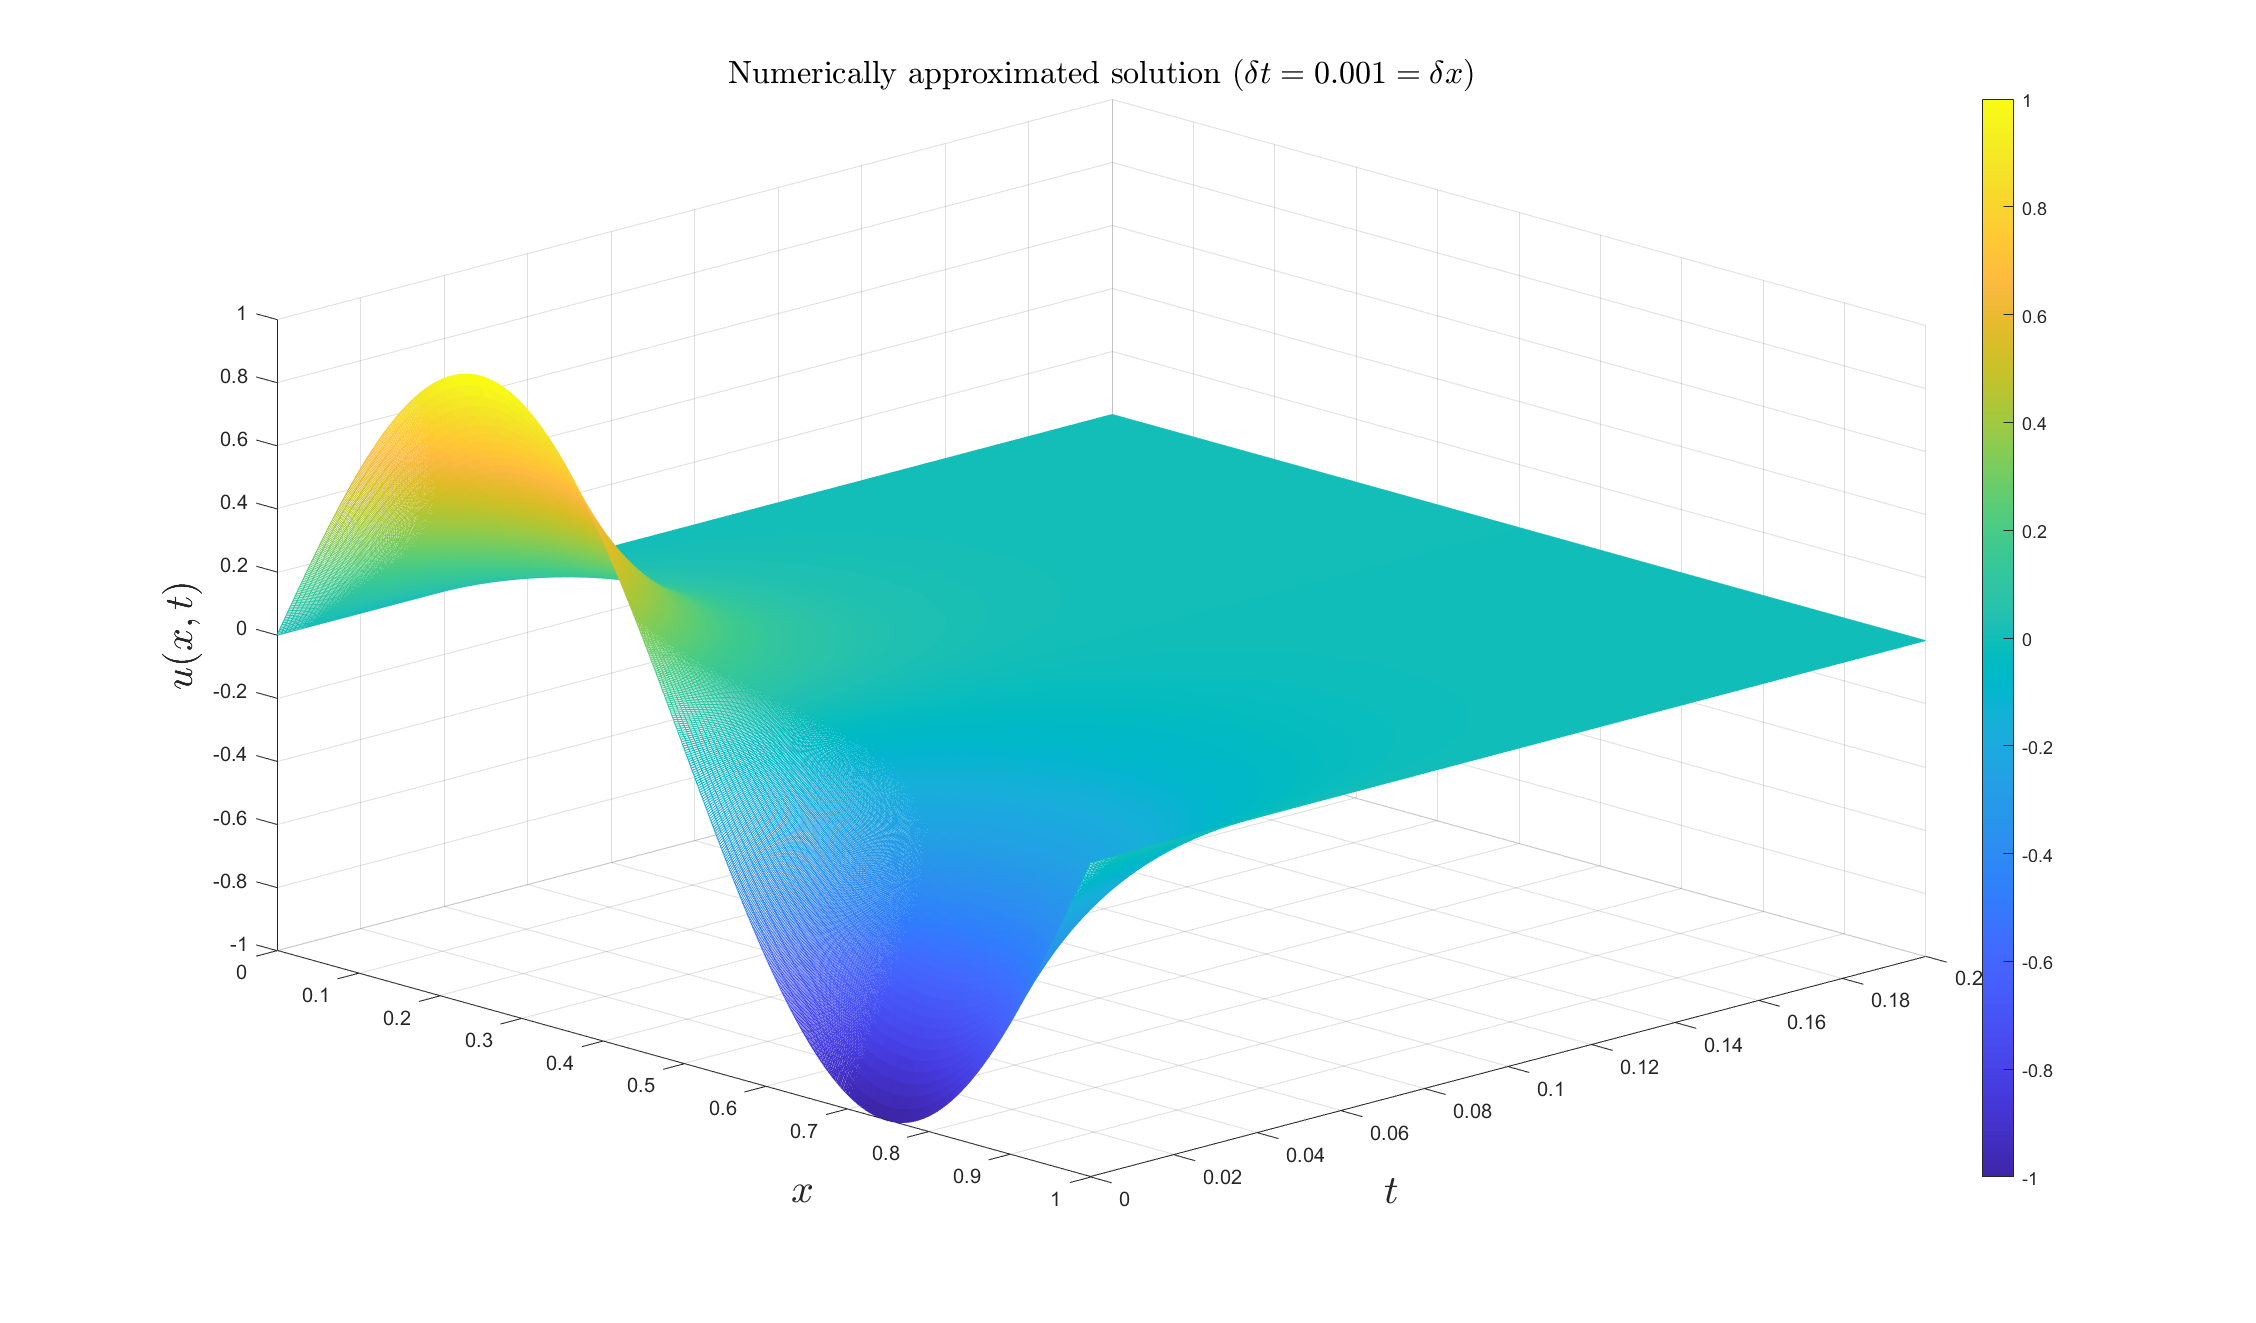
\includegraphics[scale = 0.25]{wave_eq_sol_numerical.png}
    \end{center}
    To numerically approximate the integral ${\displaystyle \int_0^1 \sin(2\pi x)\sin(n\pi x) dx }$, since the integrand $f(x) = \sin(2\pi x)\sin(n \pi x)$ is periodic on $[0,1]$, we use the trapezoidal rule for spectral accuracy. Further, 100 terms in the Fourier series were kept.
    

    \end{itemize}
    
\end{itemize}

\end{document}
